\documentclass[a4paper, 11pt]{article}
\usepackage{{../../paquete}}
\usepackage{{../../estilos}}
\graphicspath{{../Figuras/}} %Esta es la forma en la que se insertan direcciones RELATIVAS ya que la carpeta Figuras y el documento se encuentran en la misma ubicación


\newcommand{\nombreMateria}{Electrónica Industrial}


\begin{document}
	\ProvidesPackage{portada}

\usepackage{tikz}
\usepackage{setspace}
\definecolor{maincolor}{HTML}{213250}

\makeatletter
\renewcommand{\maketitle}{
	\begin{titlepage}\centering
		\begin{tikzpicture}[remember picture, overlay]
			\draw[line width=60pt, color=maincolor] 
			([xshift=1cm, yshift=-1cm]current page.north west) 
			rectangle 
			([xshift=-1cm, yshift=1cm]current page.south east);
		\end{tikzpicture}
		\vfill
		
\includegraphics[width=4cm]{recursos/logo}\\[5pt]
		{\Large \textsc{Universidad Tecnológica Nacional}\\[5pt]
			Facultad Regional Reconquista\\[5pt]
			Ingeniería Electromecánica}\\[3cm]
		
		\begin{minipage}{.7\linewidth}
			\centering
			\setstretch{.9}
			{\Huge\textbf{\@title}\\[5pt]
				\LARGE \emph{Apunte de Cátedra} \par}
			\vspace{3cm}
		\end{minipage}
		\vfill
		{\@author\\[5pt]
			\large \@date}
		\vfill
	\end{titlepage}
}
\makeatother

	\pagestyle{fancy}
	\section{Dispositivos de estado sólido}
\subsection{Diodos semiconductores}

Los diodos semiconductores son dispositivos electrónicos que permiten que \textbf{la corriente eléctrica fluya en una sola dirección}, mientras que en la dirección opuesta impide el paso. Están fabricados a partir de materiales semiconductores, como el \textsl{silicio} o el \textsl{germanio}, que tienen una conductividad eléctrica intermedia entre los conductores y los aislantes.\\


El diodo semiconductor consta de dos regiones de material semiconductor dopado con impurezas de diferentes tipos, creando así una unión \textbf{PN}. La región de tipo \textbf{P} se llama ánodo, mientras que la región de tipo \textbf{N} se llama cátodo.

Cuando se aplica una tensión en la dirección correcta (es decir, en la dirección ánodo-cátodo), los electrones se mueven a través de la unión PN y fluyen a través del diodo, lo que permite que la corriente eléctrica pase a través del dispositivo. Sin embargo, cuando se aplica una diferencia de potencial en la dirección opuesta, la unión PN actúa como una barrera y la corriente eléctrica se bloquea.

Los diodos semiconductores se utilizan en una amplia variedad de aplicaciones, como la rectificación de corriente eléctrica de CA a CC, la protección contra sobretensiones, la regulación de voltaje y la generación de luz en diodos emisores de luz (LED). Además, se utilizan en dispositivos más complejos, como los transistores y los circuitos integrados.

\subsubsection{Curva característica}

La curva característica de un diodo es una representación gráfica de la relación entre la corriente y la tensión que fluyen a través del diodo en diferentes condiciones de operación.\\


El diodo de tipo PN tiene una curva que se muestra en la figura \ref{fig:cc-diodo-pn} y pueden observarse dos zonas:
\begin{itemize}
	\item \textsl{Zona de polarización directa:} el ánodo tiene aplicada una mayor tensión respecto al cátodo. Si se supera una tensión $V_f$ (característica de cada dispositivo), el diodo conduce corriente.
	\item \textsl{Zona de polarización inversa:} el cátodo tiene aplicada una mayor tensión respecto al ánodo. El diodo no conducirá corriente siempre y cuando no supere la \textsl{tensión de ruptura} o \textsl{tensión pico inversa}.
\end{itemize} 

\subsection{Diodos Zener}

Un diodo Zener es un tipo especial de diodo que \textbf{se utiliza para regular la tensión en un circuito electrónico}. A diferencia de los diodos regulares, que sólo permiten el flujo de corriente en una dirección, los diodos Zener están diseñados para \textbf{permitir el flujo de corriente en ambas direcciones} cuando la tensión aplicada alcanza un valor específico llamado \textsl{tensión de ruptura} o \textsl{tensión Zener}.\\

\begin{figure}[H]
	\centering
	\begin{subfigure}[b]{.3\linewidth}
		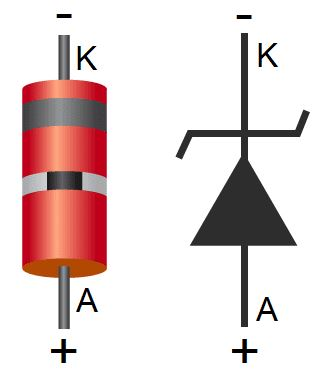
\includegraphics[width = .8\linewidth]{zener-directa}
		\caption{En directa}
		\label{fig:zener-directa}
	\end{subfigure}
	\begin{subfigure}[b]{.3\linewidth}
		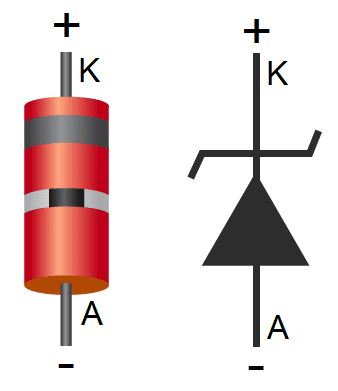
\includegraphics[width = .8\linewidth]{zener-inversa}
		\caption{En inversa}
		\label{fig:zener-inversa}
	\end{subfigure}
	\caption{Polarización del diodo zener}
\end{figure}


Cuando un diodo Zener está polarizado en inversa, como ilustra la figura \ref{fig:zener-inversa}, y se alcanza la tensión Zener, comienza a conducir corriente en la dirección opuesta, lo que permite que la tensión se mantenga constante en el circuito.

 Debido a esta propiedad, los diodos Zener se utilizan comúnmente en aplicaciones de regulación de voltaje, como fuentes de alimentación, reguladores de voltaje y circuitos de protección contra sobretensiones.
	\section{Transistores}

faltan los tipos y eso... lo vimos en una clase, aunque dijo el profesor que no ibamos a verlos, solo los mencionaba, de todas maneras, no estaría demás mencionarlo nosotros también... o qué consideran?
\subsection{Transistores bipolares}

introducción?
\subsubsection{Construcción}


En la construcción de los transistores hoy en día se emplean materiales como germanio (Ge), silicio (Si), arseniuro de galio (GaAs) o aleaciones de silicio y germanio o silicio y aluminio.

El material es dopado con otras sustancias que le permitan tener un exceso de electrones o un déficit de los mismos (vacantes
), para así formar capas en forma de ``sandwich''.\\



Por ejemplo, para el caso del Silicio mostrado en la figura \ref{fig:silicio} si es dopado con Fósforo (P) (extremo derecho de la \ref{fig:silicio-dopado}), por cada átomo de fósforo existirá un electrón excedente; si es dopado con Aluminio (Al), existirá una vacante (extremo izquierdo de la \ref{fig:silicio-dopado}).


Este juego entre electrones excedentes y vacantes representa el funcionamiento principal de los transistores bipolares.


\begin{figure}[H]
	\centering
	\begin{subfigure}[b]{.45\linewidth}
		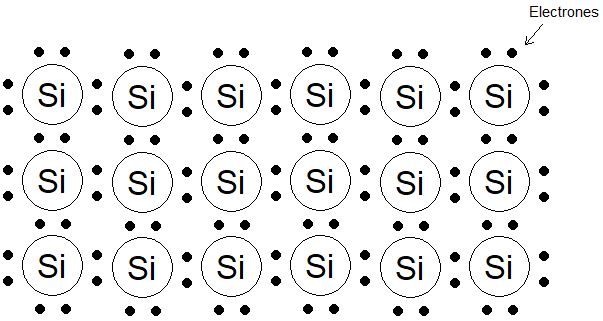
\includegraphics[width=\linewidth]{silicio}
		\caption{Silicio sin dopar}
		\label{fig:silicio}
	\end{subfigure}
	\begin{subfigure}[b]{.45\linewidth}
		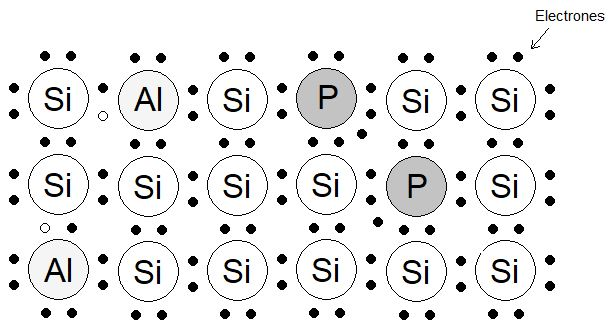
\includegraphics[width=\linewidth]{silicio-dopaje}
		\caption{Silicio dopado}
		\label{fig:silicio-dopado}
	\end{subfigure}
\end{figure}



Cuando el material tiene un excedente de electrones se dice que es \textsl{tipo n}, y cuando tiene vacantes es de \textsl{tipo p}. Con esto en mente, existen dos configuraciones en la construcción de un transistor:

\begin{itemize}
	\item \textbf{pnp:} dos capas externas de material tipo p y una capa delgada interna de material tipo n;
	\item \textbf{npn:} dos capas externas de material tipo n y una capa delgada interna de material tipo p.
\end{itemize}

\begin{figure}[H]
	\centering
	\begin{subfigure}[b]{.4\linewidth}
		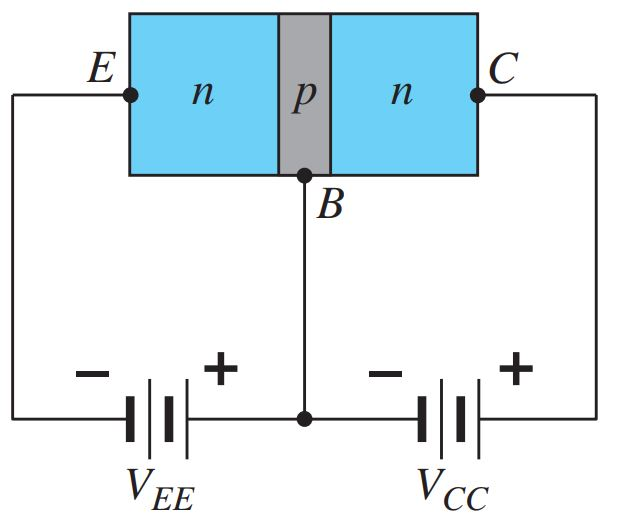
\includegraphics[width= .9\linewidth]{npn}
		\caption{Tipo NPN}
	\end{subfigure}
	\begin{subfigure}[b]{.4\linewidth}
		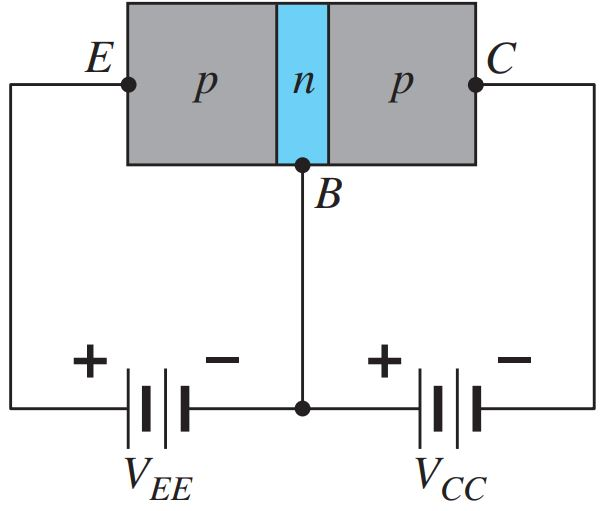
\includegraphics[width= .9\linewidth]{pnp}
		\caption{Tipo PNP}
	\end{subfigure}
	\caption{Transistores bipolares}
	\label{fig:transistores}
\end{figure}

Con la polarización mostrada en la figura \ref{fig:transistores}, las terminales se identificaron por medio de las
letras mayúsculas E para \textsl{emisor}, C para \textsl{colector} y B para \textsl{base}.\\

La capa del emisor está muy dopada, la base ligeramente, y el colector está moderadamente dopado, más que la base y menos que el emisor. \\
(Propósito de por qué ese dopaje)

\subsubsection{Union pn}

En los transistores hay dos uniones pn.\\

Tension que se forma en la unión.
Para el silicio, 0,7V...\\

Falta completar

\subsubsection{Ganancia de corriente $\beta$}

\begin{equation}
	\beta = \dfrac{i_C}{i_B}
\end{equation}
	
\end{document}